
%(BEGIN_QUESTION)
% Copyright 2011, Tony R. Kuphaldt, released under the Creative Commons Attribution License (v 1.0)
% This means you may do almost anything with this work of mine, so long as you give me proper credit

Write an equation describing the output voltage as a function of temperature, assuming the RTD (Resistive Temperature Detector) has a resistance predicted by the following formula:

$$R_{RTD} = 100 (1 + 0.00392T)$$

$$\includegraphics[width=15.5cm]{i00536x01.eps}$$

\vskip 30pt

$V_{out} = f(T) = $

\vfil 

\underbar{file i00536}
\eject
%(END_QUESTION)





%(BEGIN_ANSWER)

This is a graded question -- no answers or hints given!

%(END_ANSWER)





%(BEGIN_NOTES)

The voltage divider formula gives us an expression solving for a resistor's voltage drop given source voltage and resistor values:

$$V_{R1} = V_{source} \left(R_1 \over R_1 + R_2 \right)$$

In this example, the RTD is resistance $R_1$ and the fixed 1 k$\Omega$ resistor is $R_2$, so:

$$V_{out} = 5 \left(R_{RTD} \over R_{RTD} + 1000 \right)$$

What we need to do now is substitute the RTD resistance formula everwhere we see $R_{RTD}$ in the above equation, and then simplify the expression:

$$V_{out} = 5 \left(100(1 + 0.00392T) \over 100(1 + 0.00392T) + 1000 \right)$$

$$V_{out} = 5 \left(100 + 0.392T \over 100 + 0.392T + 1000 \right)$$

\vskip 10pt

$$V_{out} = 5 \left({100 + 0.392 T} \over {1100 + 0.392 T}\right)$$

%INDEX% Mathematics review: substituting equations

%(END_NOTES)


